% 12. Develop a LaTeX script to create a simple report and article using suitable commands
% and formats

\documentclass[a4paper, 12pt]{report} % Document class for a report

\usepackage[utf8]{inputenc} % Input encoding
\usepackage{amsmath, amssymb} % For mathematical symbols
\usepackage{graphicx} % For including images
\usepackage{hyperref} % For hyperlinks in the document

\title{Simple Report Example}
\author{Shivakumar} % Replace with your name
\date{\today} % Date of the report

\begin{document}

\maketitle % Create the title page

\tableofcontents % Generate table of contents

\chapter{Introduction} % Chapter 1
This is the introduction of the report. In this report, we discuss several concepts, such as \LaTeX\ formatting and document structuring.

\section{Background} % Section under the chapter
This section provides background information about the report's topic.

\subsection{History of LaTeX} % Subsection under Background
LaTeX was created by Leslie Lamport in the early 1980s as a document preparation system based on Donald Knuth's TeX typesetting system.

\chapter{Methodology} % Chapter 2
In this chapter, we describe the methods and techniques used to accomplish the research presented in this report.

\section{Research Method} % Section under Methodology
The research method used is a combination of quantitative and qualitative approaches.

\chapter{Results and Discussion} % Chapter 3
This chapter discusses the findings from the research, including charts, figures, and tables.

\section{Graphical Representation} % Section under Results and Discussion
Below is a simple graphical representation:

\begin{figure}[h] % Example of including a figure
\centering
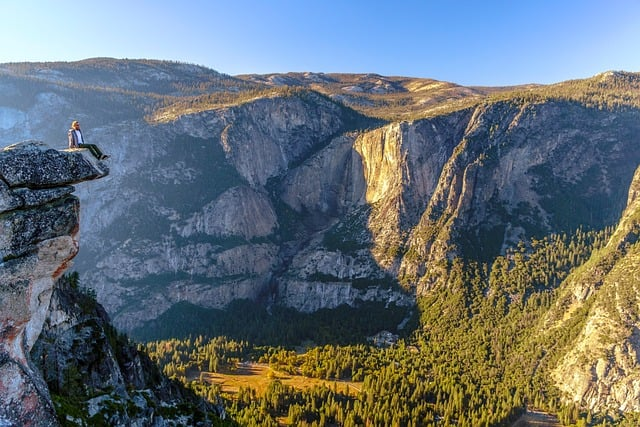
\includegraphics[width=0.5\textwidth]{image2.jpg} % Replace with your image file
\caption{Example of a Graph}
\end{figure}

\chapter{Conclusion} % Chapter 4
In this report, we have presented several concepts. The conclusion summarizes the findings and discusses future work.

\end{document}
